\section{Технический проект}
\subsection{Общая характеристика организации решения задачи}

Необходимо спроектировать и разработать фреймворк, который должен ускорить разработку графических интерфейсов и оптимизировать емкостные характеристики приложения.
Основое внимание следует уделить самым важным элементам взаимодействия с пользователем и выполняемого ими функционала.

\subsubsection{Обоснование выбора технологии проектирования}

На сегодняшний день информационный рынок, поставляющий программные решения в выбранной сфере, предлагает множество продуктов, позволяющих достигнуть поставленной цели – создание фреймворка.
В процессе разработки фреймворка используются язык программирования С++. Также, значения основных переменных задавались в json-файлах.

\subsubsection{Язык программирования С++}

С++ – это высокоуровневый язык программирования общего назначения. Этот язык программирования зарекомендовал себя, ибо уже имеет множество библиотек и фреймворков.

Преимущества использования языка C++ при создании фреймворков:
\begin{itemize}
\item Высокая производительность: C++ является компилируемым языком с низким уровнем абстракции, что позволяет создавать быстрые и эффективные фреймворки.
\item Возможность доступа к аппаратному обеспечению: C++ позволяет напрямую управлять памятью и ресурсами компьютера, что полезно при разработке фреймворков, работающих с аппаратным обеспечением.
\item Богатая функциональность: C++ обладает множеством возможностей и библиотек, что позволяет создавать мощные и гибкие фреймворки для различных целей.
\end{itemize}

Недостатки использования языка C++ при создании фреймворков:
\begin{itemize}
\item Сложность: C++ – сложный и мощный язык программирования, который требует от разработчиков высокого уровня квалификации. Это может затруднить разработку и поддержку фреймворка, особенно для менее опытных программистов.
\item Низкая гибкость: Использование C++ может привести к более жесткой архитектуре фреймворка, что может затруднить его дальнейшее развитие и модификацию.
\item Сильная типизация: C++ имеет сильную статическую типизацию, что может потребовать более тщательного и длительного процесса разработки, особенно при работе с большими проектами.
\end{itemize}

Таким образом, использование языка С++ при разработке фреймворков обладает рядом преимуществ. Во-первых, С++ является высокопроизводительным языком программирования, что позволяет создавать быстрые и эффективные фреймворки. Во-вторых, С++ обладает богатыми возможностями для объектно-ориентированного программирования, что упрощает создание модульной и расширяемой архитектуры фреймворка. Кроме того, С++ поддерживает многопоточность, что позволяет улучшить производительность и масштабируемость фреймворка. В целом, использование языка С++ при разработке фреймворков позволяет создавать мощные, гибкие и эффективные инструменты для разработки программного обеспечения.

\subsubsection{Cравнение методов отрисовки компонетов}

GDI+ (Graphics Device Interface+) - это набор API для отрисовки 2D графики в операционной системе Windows. Он предоставляет набор простых методов для рисования примитивов, текста, изображений и других графических элементов. GDI+ поддерживает аппаратное ускорение графики и имеет удобный интерфейс для работы с изображениями. Однако он ограничен в возможностях 3D графики.

OpenGL\cite{gl} - это кросс-платформенная библиотека для отображения 2D и 3D графики. Она предоставляет низкоуровневый доступ к графическому аппарату компьютера и поддерживает широкий спектр возможностей, включая шейдеры, текстурирование, освещение и другие эффекты. OpenGL позволяет создавать более сложные и реалистичные графические эффекты, чем GDI+, но требует более глубокого понимания работы с графикой.

Vulkan\cite{vulkan} - это новое поколение библиотеки для написания графических приложений, разработанное компанией Khronos Group. Она предоставляет низкоуровневый доступ к графическому аппарату и позволяет максимально эффективно использовать мощности современных GPU. Vulkan обеспечивает высокую производительность и позволяет параллельно обрабатывать большое количество графических команд. Однако для работы с ней требуется глубокое знание графического программирования.

При создании графических интерфейсов для приложений можно использовать любой из указанных методов в зависимости от требуемого уровня сложности и производительности. GDI+ подходит для простых 2D интерфейсов, OpenGL позволяет создавать более сложные 2D и 3D графику, а Vulkan обеспечивает высокую производительность и возможности для создания сложных 3D интерфейсов. Из-за своей простоты я выбрал Graphics Device Interface+.

\subsubsection{Достоинства Json}

JSON (JavaScript Object Notation) - это легкий формат обмена данными, основанный на тексте, который используется для передачи структурированных данных между программами.

Преимущества JSON:
\begin{itemize}
\item простота использования: JSON легко читаем и понятен людям, что делает его удобным для работы с данными;
\item легкость: JSON файлы компактны и занимают мало места, что ускоряет передачу данных и уменьшает нагрузку на сеть;
\item поддержка множества языков программирования: JSON поддерживается большинством языков программирования, что делает его универсальным форматом для обмена данными между различными системами;
\item поддержка структурированных данных: JSON поддерживает различные типы данных, включая строки, числа, логические значения, массивы и объекты, что позволяет передавать сложные структуры данных;
\item гибкость: JSON позволяет легко добавлять, изменять и удалять данные, а также манипулировать ими, что делает его удобным для работы с динамическими данными.
\end{itemize}
Таким образом, использование JSON упрощает обмен данными между различными системами и позволяет эффективно передавать информацию в формате, который легко читать и понять.

\subsection{Диаграмма компонентов и схема обмена данными между классами}

Диаграмма компонентов описывает особенности физического представления разрабатываемой системы. Она позволяет определить архитектуру системы, установив зависимости между программными компонентами, в роли которых может выступать как исходный, так и исполняемый код. Основными графическими элементами диаграммы компонентов являются классы, а также зависимости между ними. На рисунке \ref{comp:image} изображена диаграмма компонентов для проектируемой системы. Она базируется на двух сущностях - Window и Control. Окно может содержать контролы, также само окно является контролом.

\begin{figure}[H]
\center{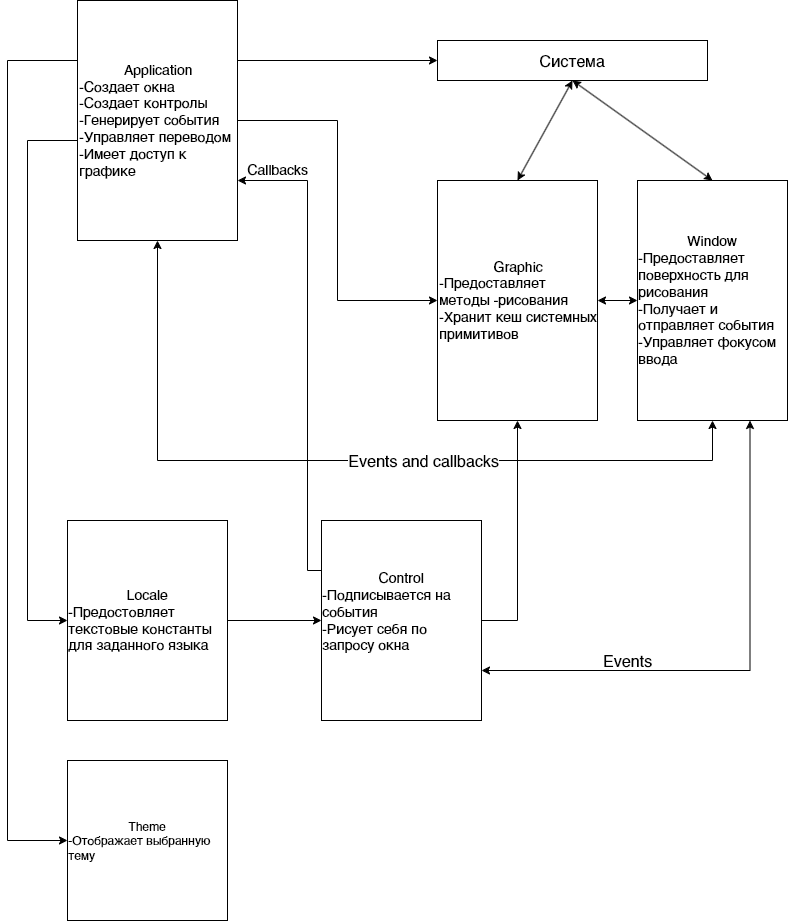
\includegraphics[width=1\linewidth]{comp}}
\caption{Cхема обмена данными между классами}
\label{comp:image}
\end{figure}

\subsection{Описание основных сущностей}

Проанализировав требования, можно выделить девять основных сущностей:
\begin{itemize}
\item "<Фреймворк">;
\item "<Окно">;
\item "<Компонент">;
\item "<Кнопка">;
\item "<Изображение">;
\item "<Графика">;
\item "<Тема">;
\item "<Локаль">;
\item "<Ошибка">.
\end{itemize}

В состав сущности "<Фреймворк"> можно включить атрибуты, представленные в таблице \ref{framework_a:table}.

\begin{xltabular}{\textwidth}{|l|l|p{1.7cm}|X|}
	\caption{Атрибуты сущности "<Фреймворк">\label{framework_a:table}}\\ \hline
	\centrow Поле & \centrow Тип & \centrow Обяза\-тельное & \centrow Описание \\ \hline
	\thead{1} & \thead{2} & \centrow 3 & \centrow 4 \\ \hline
	\endfirsthead
	\continuecaption{Продолжение таблицы \ref{framework_a:table}}
	\thead{1} & \thead{2} & \centrow 3 & \centrow 4 \\ \hline
	\finishhead
	\ runned & bool & false & Флаг запуска приложения \\ \hline
	err & error & false & Ошибка
\end{xltabular}

В состав сущности "<Ошибка"> можно включить атрибуты, представленные в таблице \ref{error_a:table}.

\begin{xltabular}{\textwidth}{|l|l|p{1.7cm}|X|}
	\caption{Атрибуты сущности "<Ошибка">\label{error_a:table}}\\ \hline
	\centrow Поле & \centrow Тип & \centrow Обяза\-тельное & \centrow Описание \\ \hline
	\thead{1} & \thead{2} & \centrow 3 & \centrow 4 \\ \hline
	\endfirsthead
	\continuecaption{Продолжение таблицы \ref{error_a:table}}
	\thead{1} & \thead{2} & \centrow 3 & \centrow 4 \\ \hline
	\finishhead
	\ type & error{\_}type & true & тип ошибки \\ \hline
	component & string & true & указатель на компонент, вызвавший ошибку \\ \hline
	message & string & true & Сообщение \\ \hline
\end{xltabular}

В состав сущности "<Графика"> можно включить атрибуты, представленные в таблице \ref{graphic_a:table}.

\begin{xltabular}{\textwidth}{|l|l|p{1.7cm}|X|}
	\caption{Атрибуты сущности "<Графика">\label{graphic_a:table}}\\ \hline
	\centrow Поле & \centrow Тип & \centrow Обяза\-тельное & \centrow Описание \\ \hline
	\thead{1} & \thead{2} & \centrow 3 & \centrow 4 \\ \hline
	\endfirsthead
	\continuecaption{Продолжение таблицы \ref{graphic_a:table}}
	\thead{1} & \thead{2} & \centrow 3 & \centrow 4 \\ \hline
	\finishhead
	\ pc & primitive{\_}container & true & Примитивный контейнер для хранения \\ \hline
	max{\_}size & rect & true & максимальный размер \\ \hline
	background{\_}color & color & true & Задний фон \\ \hline
	mem{\_}dc & HDC & true & Указатель на графический объект \\ \hline
	mem{\_}bitmap & HBITMAP & true & Указатель на битмап \\ \hline
	err & error & false & Ошибка
\end{xltabular}

В состав сущности "<Компонент"> можно включить атрибуты, представленные в таблице \ref{control_a:table}.

\begin{xltabular}{\textwidth}{|l|l|p{1.7cm}|X|}
	\caption{Атрибуты сущности "<Компонент">\label{control_a:table}}\\ \hline
	\centrow Поле & \centrow Тип & \centrow Обяза\-тельное & \centrow Описание \\ \hline
	\thead{1} & \thead{2} & \centrow 3 & \centrow 4 \\ \hline
	\endfirsthead
	\continuecaption{Продолжение таблицы \ref{control_a:table}}
	\thead{1} & \thead{2} & \centrow 3 & \centrow 4 \\ \hline
	\finishhead
	\_position & rect & true & Позиция элемента \\ \hline
	parent & window & true & Родительское окно \\ \hline 
	topmost & bool & true & Флаг "<Поверх всех элементов"> \\ \hline 
	showed & bool & true & Видимость элемента \\ \hline 
	enabled & bool & true & Включенность элемента \\ \hline 
	focused & bool & false & Возвращает true, если элемент управления сфокусирован \\ \hline 
	focusing & bool & false & Возвращает true, если элемент управления получает фокус \\ \hline
	err & error & false & Ошибка
\end{xltabular}

В состав сущности "<Компонент Кнопка"> можно включить атрибуты, представленные в таблице \ref{button_a:table}.

\begin{xltabular}{\textwidth}{|l|l|p{1.7cm}|X|}
	\caption{Атрибуты сущности "<Кнопка">\label{button_a:table}}\\ \hline
	\centrow Поле & \centrow Тип & \centrow Обяза\-тельное & \centrow Описание \\ \hline
	\thead{1} & \thead{2} & \centrow 3 & \centrow 4 \\ \hline
	\endfirsthead
	\continuecaption{Продолжение таблицы \ref{button_a:table}}
	\thead{1} & \thead{2} & \centrow 3 & \centrow 4 \\ \hline
	\finishhead
	\ button{\_}view{\_} & button{\_}view & true & Вид кнопки \\ \hline
	caption & string & true & Надпись на кнопке \\ \hline
	image{\_} & string & false & Изображение на кнопке \\ \hline
	image{\_}size & int32{\_}t & false & Размер изображения \\ \hline
	tooltip{\_} & tooltip & false & Подсказка при наведения на кнопку \\ \hline
	theme{\_}  & i{\_}theme & true & Тема кнопки \\ \hline
	{\_}position & rect & true & Позиция элемента \\ \hline
	parent & window & true & Родительское окно \\ \hline
	my{\_}subscriber{\_}id & string & true & Подписка на события \\ \hline
	topmost & bool & true & Флаг "<Поверх всех элементов"> \\ \hline 
	pushed, turned & bool & false & Флаг "<Включения кнопки"> \\ \hline 
	showed & bool & true & Видимость элемента \\ \hline 
	enabled & bool & true & Включенность \\ \hline 
	focused & bool & false & Возвращает true, если элемент управления сфокусирован \\ \hline 
	focusing & bool & false & Возвращает true, если элемент управления получает фокус \\ \hline
	err & error & false & Ошибка
\end{xltabular}

В состав сущности "<Компонент Изображение"> можно включить атрибуты, представленные в таблице \ref{img_a:table}.

\begin{xltabular}{\textwidth}{|l|l|p{1.7cm}|X|}
	\caption{Атрибуты сущности "<Изображение">\label{img_a:table}}\\ \hline
	\centrow Поле & \centrow Тип & \centrow Обяза\-тельное & \centrow Описание \\ \hline
	\thead{1} & \thead{2} & \centrow 3 & \centrow 4 \\ \hline
	\endfirsthead
	\continuecaption{Продолжение таблицы \ref{img_a:table}}
	\thead{1} & \thead{2} & \centrow 3 & \centrow 4 \\ \hline
	\finishhead
	\ img{\_} & Gdiplus::Image & true & Полотно изображения \\ \hline
	file{\_}name & string & true & Имя изображения \\ \hline
	resource{\_}index & int32{\_}t & true & Индекс ресурса \\ \hline
	theme{\_}  & i{\_}theme & true & Тема изображения \\ \hline
	{\_}position & rect & true & Позиция изображения \\ \hline
	parent & window & true & Родительское окно \\ \hline
	topmost & bool & true & Флаг "<Поверх всех элементов"> \\ \hline 
	showed & bool & true & Видимость элемента \\ \hline  
	err & error & false & Ошибка
\end{xltabular}

В состав сущности "<Окно"> можно включить атрибуты, представленные в таблице \ref{window_a:table}.

\begin{xltabular}{\textwidth}{|l|l|p{1.7cm}|X|}
	\caption{Атрибуты сущности "<Окно">\label{window_a:table}}\\ \hline
	\centrow Поле & \centrow Тип & \centrow Обяза\-тельное & \centrow Описание \\ \hline
	\thead{1} & \thead{2} & \centrow 3 & \centrow 4 \\ \hline
	\endfirsthead
	\continuecaption{Продолжение таблицы \ref{window_a:table}}
	\thead{1} & \thead{2} & \centrow 3 & \centrow 4 \\ \hline
	\finishhead
	\ graphic{\_} & rect & true & Полотно для рисования \\ \hline
	controls & std::vector & true & Компоненты окна \\ \hline
	active{\_}control & i{\_}control & true & Активный компонент \\ \hline
	caption & string & true & Название окна \\ \hline
	{\_}position, normal{\_}position & rect & true & Позиция окна \\ \hline
	min{\_}width, min{\_}height & int32{\_}t & true & Минимальная высота/ширина окна \\ \hline
	window{\_}style{\_} &  window{\_}style & true & Тип окна \\ \hline
	window{\_}state{\_}, prev{\_}window{\_}state{\_} & window{\_}state & true & Состояние окна \\ \hline
	theme{\_} & i{\_}theme & true & Тема окна \\ \hline
	showed & bool & true & Видимость окна \\ \hline  
	skip{\_}draw{\_} & bool & true & Флаг пропуска отрисовки \\ \hline
	focused & bool & false & Фокус\\ \hline 
	docked{\_} & bool & false & Флаг прикрепления к окну \\ \hline 
	docked{\_}control & i{\_}control & false & Прикреп-\ ленный к окну элемент \\ \hline 
	subscribers{\_} & std::vector & false & Подписанные на события элементы \\ \hline
	mouse{\_}tracked & bool & false & Флаг отслеживания мыши \\ \hline
	x{\_}click, y{\_}click & int16{\_}t & false & Координаты клика \\ \hline 
	switch{\_}lang{\_}button & button & true & Кнопка управления языком \\ \hline
	switch{\_}theme{\_}button & button & true & Кнопка управления темой \\ \hline
	pin{\_}button & button & true & Кнопка управления закреплением \\ \hline
	minimize{\_}button & button & true & Кнопка "<Свернуть"> \\ \hline
	expand{\_}button & button & true & Кнопка "<Расширить"> \\ \hline
	close{\_}button & button & true & Кнопка "<Закрыть"> \\ \hline
	err & error & false & Ошибка
\end{xltabular}

В состав сущности "<Локаль"> можно включить атрибуты, представленные в таблице \ref{locale_a:table}.

\begin{xltabular}{\textwidth}{|l|l|p{1.7cm}|X|}
	\caption{Атрибуты сущности "<Локаль">\label{locale_a:table}}\\ \hline
	\centrow Поле & \centrow Тип & \centrow Обяза\-тельное & \centrow Описание \\ \hline
	\thead{1} & \thead{2} & \centrow 3 & \centrow 4 \\ \hline
	\endfirsthead
	\continuecaption{Продолжение таблицы \ref{locale_a:table}}
	\thead{1} & \thead{2} & \centrow 3 & \centrow 4 \\ \hline
	\finishhead
	\ type & locale{\_}type & true & Код языка\\ \hline
	name & string & true & Название \\ \hline 
	strings & std::map & true & Строки перевода \\ \hline 
	dummy{\_}string & string & true & Строка по умолчанию \\ \hline 
	err & error & false & Ошибка
\end{xltabular}

В состав сущности "<Тема"> можно включить атрибуты, представленные в таблице \ref{theme_a:table}.

\begin{xltabular}{\textwidth}{|l|l|p{1.7cm}|X|}
	\caption{Атрибуты сущности "<Тема">\label{theme_a:table}}\\ \hline
	\centrow Поле & \centrow Тип & \centrow Обяза\-тельное & \centrow Описание \\ \hline
	\thead{1} & \thead{2} & \centrow 3 & \centrow 4 \\ \hline
	\endfirsthead
	\continuecaption{Продолжение таблицы \ref{theme_a:table}}
	\thead{1} & \thead{2} & \centrow 3 & \centrow 4 \\ \hline
	\finishhead
	\ type & locale{\_}type & true & Код языка\\ \hline
	name & string & true & Название \\ \hline 
	ints & std::map & true & Коллекция чисел \\ \hline
	strings & std::map & true & Строки \\ \hline
	fonts & std::map & true & Коллекция шрифтов \\ \hline
	imgs & std::map & true & Коллекция изображений \\ \hline
	dummy{\_}string & string & true & Строка по умолчанию \\ \hline
	dummy{\_}image & std::vector<uint8{\_}t> & true & Изображение по умолчанию \\ \hline 
	err & error & false & Ошибка
\end{xltabular}

В системе предусмотрен внутренний механизм связи между разделами и элементами информационных блоков, поэтому введения дополнительных идентификаторов при реализации связей между сущностями не предполагается.

Экземпляры сущностей реализуются в информационных блоках посредством элементов, атрибуты сущности – посредством полей и свойств элемента. 

\subsection{Описание сущностей для настройки окна}

В состав сущности "<Тема"> можно включить набор основных полей JSON-документа и их описание, представленные в таблице \ref{json-theme:table}.


\begin{xltabular}{\textwidth}{|X|>{\setlength{\baselineskip}{0.7\baselineskip}}p{4.85cm}|>{\setlength{\baselineskip}{0.7\baselineskip}}p{4.85cm}|}
	\caption{Описание полей JSON-документа сущности "<Тема">\label{json-theme:table}}\\
	\hline \centrow \setlength{\baselineskip}{0.7\baselineskip} Ключ & \centrow Тип & \centrow Описание \\
	\hline \centrow 1 & \centrow 2 & \centrow 3 \\ \hline
	\endfirsthead
	\caption*{Продолжение таблицы \ref{json-theme:table}}\\
	\hline \centrow 1 & \centrow 2 & \centrow 3 \\ \hline
	\finishhead
	controls & map & Элементы управления \\ \hline
	type & str & Тип элемента управления \\ \hline
	background & str & Цвет заднего фона \\ \hline
	border & str & Цвет обводки  \\ \hline
	border{\_}width & number & Ширина обводки \\ \hline
	round & number & Округление \\ \hline
	text & str & Цвет текста \\ \hline
	caption{\_}font & map & Шрифт заголовка \\ \hline
	name & str & Название шрифта \\ \hline
	size & number & Размер шрифта \\ \hline
	color & str & Цвет заливки \\ \hline
	resource & str & Название ресурса \\ \hline
	path & str & Путь к папке \\ \hline
	calm & str & Основной цвет \\ \hline
	active & str & Активный цвет \\ \hline
	focused{\_}border & str & Цвет обводки при фокусировке \\ \hline
	disabled & str & Цвет при недоступности \\ \hline
	anchor & str & Цвет ссылки \\ \hline
	focusing & number & фокусировка \\ \hline
	selection & str & Цвет при выборе поля ввода \\ \hline
	button{\_}calm & str & Основной цвет кпонки при выборе клавиатурой \\ \hline
	button{\_}active & str & Цвет активированной кнопки при выборе клавиатурой \\ \hline
	scrollbar & str & Цвет полосы прокрутки \\ \hline
	scrollbar{\_}slider & str & Цвет ползунка полосы прокрутки \\ \hline
	scrollbar{\_}slider{\_}active & str & Цвет активного ползунка полосы прокрутки \\ \hline
	selected{\_}item & str & Цвет выбранного элемента \\ \hline
	active{\_}item & str & Цвет активного элемента \\ \hline
	title & str & Цвет заголовка листа \\ \hline
	title{\_}text & str & Цвет текста заголовка листа \\ \hline
	slider & str & Цвет ползунка \\ \hline
	slider{\_}active & str & Цвет активного ползунка \\ \hline
	disabled{\_}text & str & Цвет неактивного текста в меню \\ \hline
	text{\_}indent & number & Отступ текста \\ \hline
	meter & str & Цвет полосы прогресса \\ \hline
	perform & str & Цвет активной части ползунка настройки \\ \hline
	remain & str & Цвет неактивной части ползунка настройки  \\ \hline
	slider{\_}width & number & Ширина ползунка настройки \\ \hline
	slider{\_}height & number & Высота ползунка настройки \\ \hline
	images & map & Иконки окна
\end{xltabular}

В состав сущности "<Язык"> можно включить набор основных полей JSON-документа и их описание, представленные в таблице \ref{json-locale:table}.


\begin{xltabular}{\textwidth}{|X|>{\setlength{\baselineskip}{0.7\baselineskip}}p{4.85cm}|>{\setlength{\baselineskip}{0.7\baselineskip}}p{4.85cm}|}
	\caption{Описание полей JSON-документа сущности "<Тема">\label{json-locale:table}}\\
	\hline \centrow \setlength{\baselineskip}{0.7\baselineskip} Ключ & \centrow Тип & \centrow Описание \\
	\hline \centrow 1 & \centrow 2 & \centrow 3 \\ \hline
	\endfirsthead
	\caption*{Продолжение таблицы \ref{json-locale:table}}\\
	\hline \centrow 1 & \centrow 2 & \centrow 3 \\ \hline
	\finishhead
	sections & map & Элементы управления \\ \hline
	type & str & Тип элемента управления \\ \hline
	ok & str & Подтверждение \\ \hline
	yes & str & Да  \\ \hline
	no & str & Нет \\ \hline
	cancel & number & Отмена \\ \hline
	abort & str & Отказ \\ \hline
	retry & str & Повторить \\ \hline
	ignore & str & Пропустить \\ \hline
	try{\_}continue & str & Попробовать продолжить \\ \hline
	complete & str & Готово \\ \hline
	pin & str & Прикрепить окно \\ \hline
	unpin & str & Открепить окно \\ \hline
	dark{\_}theme & str & Темная тема \\ \hline
	light{\_}theme & str & Светлая тема\\ \hline
	switch{\_}lang & str & Сменить язык \\ \hline
	copy & str & Копировать \\ \hline
	cut & str & Вырезать \\ \hline
	paste & number & Вставить \\ \hline
	undo & str & Отменить \\ \hline
	redo & str & Вернуть отмену
\end{xltabular}
